%%%%%%%%%%%%%%%%%%%%%%%%%%%%%%%%%%%%%%%%%%%%%%%%%%%%%%%%%%%%%%%%%%%%%%%%%%%%%%%%%%%%%%%%%%%%%%%%%%%
% Chapter 4 -> Experiments
% Author: Eduardo G Gusmao
%%%%%%%%%%%%%%%%%%%%%%%%%%%%%%%%%%%%%%%%%%%%%%%%%%%%%%%%%%%%%%%%%%%%%%%%%%%%%%%%%%%%%%%%%%%%%%%%%%%
\chapter{Experiments}
\label{cha:experiments}

\graphicspath{{chapter4/figs/}}

% Introduction
% TODO

% Figure - Experiment design TODO
\begin{figure}[h!]
\centering
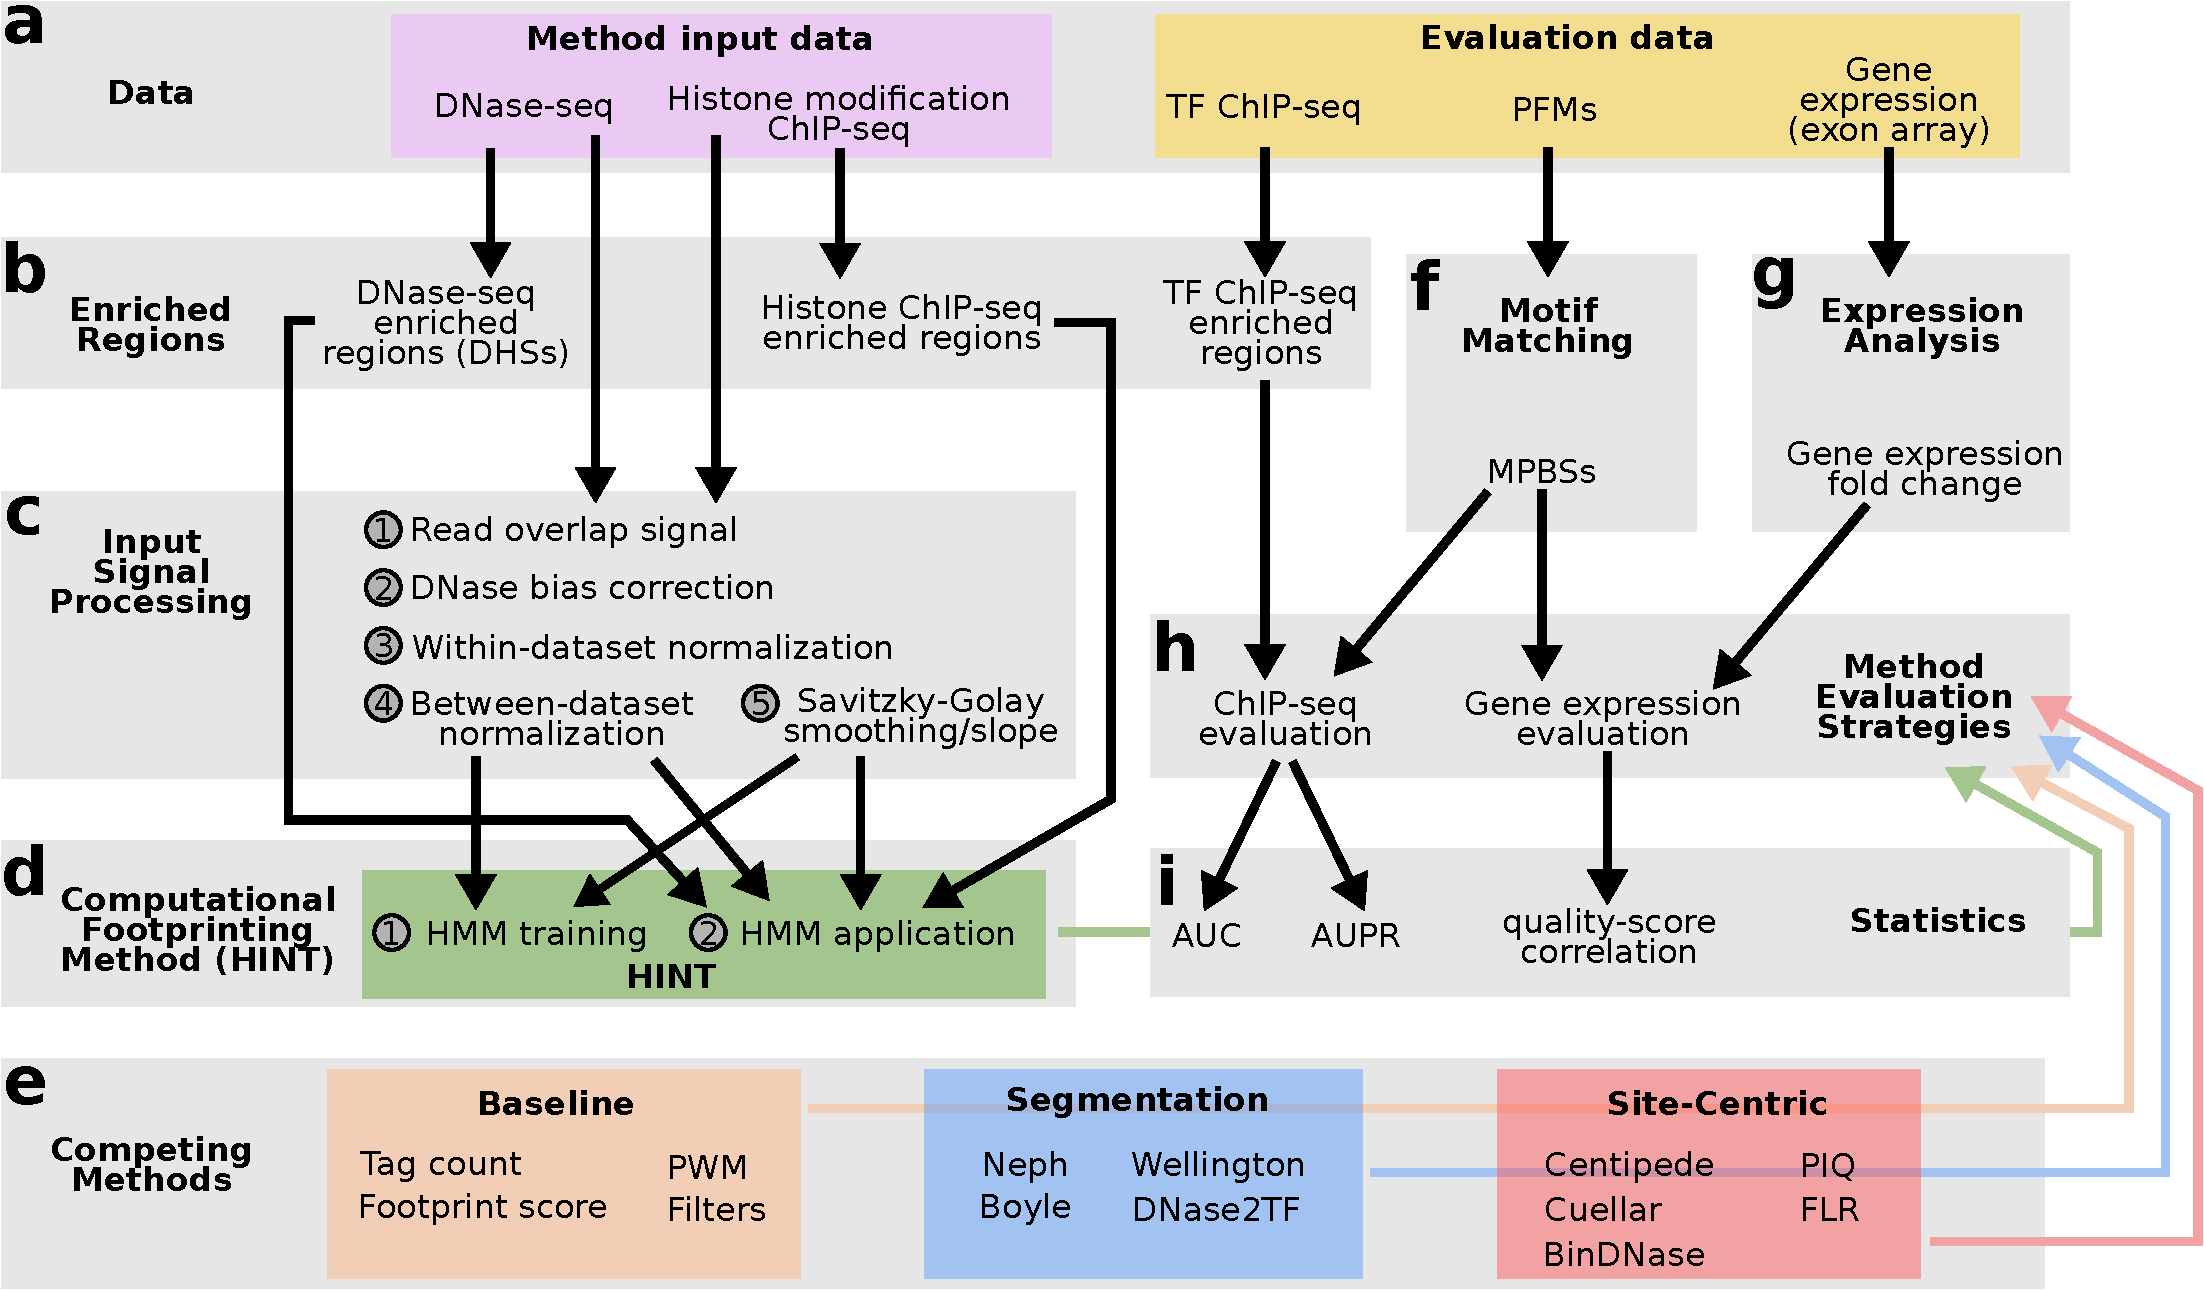
\includegraphics[width=0.99\textwidth]{gusmao_experiment_design_pipeline}
\caption[Experimental design]{\textbf{Experimental design.} Placeholder.}
\label{fig:gusmao_experiment_design_pipeline}
\end{figure}

% Parameter selection
% TODO - Falar que alguns parametros impactam na acuracia do modelo. Esses parametros serao detalhados no proximo capitulo. Falar que nesse capitulo vai dizer quais parametros sao esses.

%%%%%%%%%%%%%%%%%%%%%%%%%%%%%%%%%%%%%%%%%%%%%%%%%%%%%%%%%%%%%%%%%%%%%
% Section: Data Description
%%%%%%%%%%%%%%%%%%%%%%%%%%%%%%%%%%%%%%%%%%%%%%%%%%%%%%%%%%%%%%%%%%%%%
\section{Data Description}
\label{sec:data.description}

% Introduction
In this section we describe the data sources for this project. We state where we obtained data used: (1) as input for the computational footprinting approach (Section~\ref{sec:method.input.data}) and (2) as input for the creation of the evaluation gold standard data sets (Section~\ref{sec:evaluation.data}). The additional data required for the execution of some competing methods are described in Section~\ref{sec:competing.methods}, where we describe the experimental settings of each competing method.

% Further notes
All experimental organism-specific data (DNase-seq, ChIP-seq and gene expression) are based on the human genome build 37 (hg19), except the DNase-seq for m3134 cell and ChIP-seq for the GR transcription factor, which were based on mouse genome build 37 (mm9). Chromosome~Y was removed from all analyses. The genomic sequences (DNA) were obtained in ENCODE~\cite{encode2012}.

%%%%%%%%%%%%%%%%%%%%%%%%%%%%%%%%%%%%%%%%%%%%%%%%%%%%%%%%%%%%%%%%%%%%%
% Section: Method Input Data
%%%%%%%%%%%%%%%%%%%%%%%%%%%%%%%%%%%%%%%%%%%%%%%%%%%%%%%%%%%%%%%%%%%%%
\subsection{Method Input Data}
\label{sec:method.input.data}

% DNase-seq
DNase-seq aligned reads were obtained from ENCODE~\cite{encode2012}. To perform the computational footprint experiments, we obtained data regarding cell types H1-hESC, HeLa-S3, HepG2, Huvec, K562, LNCaP and MCF-7 from Crawford's Lab at Duke University (labeled with the initials of their institution ``DU'') and cell types H7-hESC, HepG2, Huvec, K562 and m3134 from Stamatoyannopoulous' lab at University of Washington (labeled with the initials of their institution ``UW''). We also used deproteinized DNase-seq experiments from cell types MCF-7 and K562 (Crawford lab)~\cite{yardimci2014} and IMR90 (Stamatoyannopoulous lab)~\cite{lazarovici2013}. DNase-seq experiments labeled with ``DU'' follow the single-hit DNase-seq protocol, while the experiments labeled with ``UW'' follow the double-hit DNase-seq protocol. In addition, to perform the DNase-seq bias estimation clustering, we used all cell types from ENCODE's Tier 1 and Tier 2 cell types, generated in Crawford's and Stamatoyannopoulous' labs. See Supplementary Table~\ref{tab:dataencode.dnase} for a full DNase-seq data description and accession numbers.

% Histone modifications ChIP-seq
Histone modifications ChIP-seq aligned reads were obtained from ENCODE~\cite{encode2012}. It was obtained data regarding cell types H1-hESC, HeLa-S3, HepG2 and K562 and histone modifications H3K4me1, H3K4me3, H3K9ac, H3K27ac and H2A.Z generated at the Broad Institute and in the Bernstein's lab at the Massachusetts General Hospital/Harvard Medical School. See Supplementary Table~\ref{tab:dataencode.histone} for a full histone modification ChIP-seq data description and accession numbers.

%%%%%%%%%%%%%%%%%%%%%%%%%%%%%%%%%%%%%%%%%%%%%%%%%%%%%%%%%%%%%%%%%%%%%
% Section: Evaluation Data
%%%%%%%%%%%%%%%%%%%%%%%%%%%%%%%%%%%%%%%%%%%%%%%%%%%%%%%%%%%%%%%%%%%%%
\subsection{Evaluation Data}
\label{sec:evaluation.data}

% TF ChIP-seq
All transcription factor ChIP-seq enriched regions (peaks and summits) were obtained in ENCODE Analysis Working Group (AWG) track with exception of the following experiments, in which only the raw (unaligned) DNA sequence reads were available: (1) AR (R1881 treatment) ChIP-seq raw sequences for LNCaP cell type was obtained in gene expression omnibus (GEO) with accession number GSM353644~\cite{yu2010}; (2) ER (40 and 160 minutes after estradiol treatment) ChIP-seq raw sequences for MCF-7 cell type was obtained in GEO with accession number GSE54855~\cite{guertin2014}; (3) GR (dexamethasone treatment) ChIP-seq raw sequences for m3134 cell type was obtained in the sequence read archive (SRA) under study number SRP004871~\cite{john2011}. A full description on how the enriched regions were obtained for these experiments can be found in Section~\ref{sec:chipseq.enriched.regions}. See Supplementary Table~\ref{tab:dataencode.pfm.chipseq} for a full TF ChIP-seq data description and accession numbers. This table contains information on TF ChIP-seq data and also on the TF DNA motifs associated to these TF ChIP-seq dataset for the ChIP-seq evaluation scenario (more details on Section~\ref{sec:chipseq.evaluation}).

% Gene expression data
Expression profiling by array (Affymetrix Human Exon 1.0 ST Array) data was obtained directly from GEO. It was downloaded data for cell types H1-hESC, K562 and GM12878 generated in the Microarray Core from the Center for Functional Genomics in SUNY-University at Albany. All samples from each cell type was used to infer the overall gene expression profile. See Supplementary Table~\ref{tab:data.expression} for a full gene expression data description and accession numbers.

% PFMs
TF DNA motifs represented as position frequency matrices (PFMs), were obtained from the repositories Jaspar~\cite{mathelier2014}, Uniprobe~\cite{robasky2011} and Transfac~\cite{matys2006}. These non-organism-specific data (PFMs) were obtained for the subphylum \emph{Vertebrata}. \emph{De novo} PFMs 0458 and 0500 were downloaded from Neph et al.~\cite{neph2012a}. See Supplementary Tables~\ref{tab:dataencode.pfm.chipseq} and~\ref{tab:dataencode.pfm.flrexp} for a full description on the PFMs used in this work and their IDs within their respective repositories.














%%%%%%%%%%%%%%%%%%%%%%%%%%%%%%%%%%%%%%%%%%%%%%%%%%%%%%%%%%%%%%%%%%%%%
% Section: Enriched Regions (Peak-Calling)
%%%%%%%%%%%%%%%%%%%%%%%%%%%%%%%%%%%%%%%%%%%%%%%%%%%%%%%%%%%%%%%%%%%%%
\section{Enriched Regions (Peak-Calling)}
\label{sec:enriched.regions}

% Introduction
To optimize execution time we constraint the application of our method (HINT) only in genomic regions enriched with either DNase-seq and histone modification ChIP-seq signals (more details in Section~\ref{sec:hint.application}). Furthermore, enriched regions for TF ChIP-seq are used in our evaluation methodology (more details in Section~\ref{sec:chipseq.evaluation}). In this section we describe how we obtained the enriched regions for DNase-seq data (Section~\ref{sec:dnaseseq.enriched.regions}) and the enriched regions for ChIP-seq data (Section~\ref{sec:chipseq.enriched.regions}). The process in which we identify enriched genomic signals using NGS-based data is termed peak-calling. Consequently, in many occasions we will refer to the enriched regions as peaks. We performed the identification of enriched regions on all DNase-seq and ChIP-seq data sets described in Section~\ref{sec:data.description}.

%%%%%%%%%%%%%%%%%%%%%%%%%%%%%%%%%%%%%%%%%%%%%%%%%%%%%%%%%%%%%%%%%%%%%
% Section: DNase-seq Enriched Regions
%%%%%%%%%%%%%%%%%%%%%%%%%%%%%%%%%%%%%%%%%%%%%%%%%%%%%%%%%%%%%%%%%%%%%
\subsection{DNase-seq Enriched Regions}
\label{sec:dnaseseq.enriched.regions}

% DHS estimation using F-seq
DNase I hypersensitive sites (DHSs), i.e. regions enriched with DNase-seq data, are estimated based on the DNase-seq raw (read overlap) signal $\mathbf{x}$ (Section~\ref{sec:read.overlap.signal}). The process consists on evaluating a smoothed DNase-seq signal and then finding enriched regions based on a $p$-value cutoff calculated based on a fitted Gamma distribution. The Gamma distribution was shown to outperform other models for DNase-seq data~\cite{boyle2008b}.

% F-seq, mean and variance
First, the F-seq software~\cite{boyle2008b} was used to create smoothed DNase-seq signals using Parzen density estimates. Such software was devised specially for DNase-seq data and has shown to provide accurate DHSs~\cite{boyle2008b,boyle2011}. We run the F-seq software version 1.81 with the following command. The F-seq source code, background files and ploidy files for the human genome and the specific cells we are analyzing can be also found in \url{http://fureylab.web.unc.edu/software/fseq/}.

% Software Command - F-seq
\vspace{0.3cm}
\noindent
\textbf{F-seq Software Command:}\\
\texttt{fseq -l 300 -s 1 -b [background\_file] -p [ploidy\_file] [aligned\_reads\_file] > [signal\_file]}
\vspace{0.3cm}

% Mean and variance
Then, we evaluate the mean ($\mu$) and variance ($\sigma$) of the resulting F-seq smoothed DNase-seq signal $\mathbf{x}^{\text{fseq}}$ as
\begin{align}
  \label{eq:fseq.mean.std}
  \mu &= \frac{\sum_{i=1}^{n} x^{\text{fseq}}_{i}}{n} &
  \sigma &= \frac{ \sum_{i=1}^{n} \left( x^{\text{fseq}}_{i} - \mu \right)^2}{n},
\end{align}
where $n$ is the total size of the genome.

% Gamma shape and scale
With the mean ($\mu$) and variance ($\sigma$) of the F-seq smoothed DNase-seq signal $\mathbf{x}^{\text{fseq}}$ we were able to evaluate the Gamma distribution's parameters shape ($\kappa$) and scale ($\theta$) by solving the following set of equations, which are properties of the Gamma distribution
\begin{align}
  \label{eq:fseq.shape.scale}
  \mu &= \kappa \theta &
  \sigma &= \kappa {\theta}^{2}.
\end{align}

% Gamma fit
With the shape ($\kappa$) and the scale ($\theta$) we are able to fit the F-seq smoothed signal $\mathbf{x}^{\text{fseq}}$ into a Gamma distribution, which can be written as
\begin{equation}
  \label{eq:gamma.distribution}
  \mathbf{x}^{\text{fseq}} \sim \Gamma(\kappa,\theta) = \Gamma(\mathbf{x}^{\text{fseq}}; \kappa,\theta) = 
  \frac{1}{\gamma(\kappa) {\theta}^{\kappa}} {x}^{\kappa-1} {e}^{-\frac{x}{\theta}},
\end{equation}
where $\gamma$ is the gamma function, which can be written as
\begin{equation}
  \label{eq:gamma.function}
  \gamma(t) = \int_{0}^{\infty} {x}^{t-1} {e}^{-x} \diff x
\end{equation}

% Enriched regions
The DNase-seq enriched regions (DHSs) were found by establishing a cutoff based on a $p$-value of $0.01$~\cite{boyle2008b,encode2012}. We formally refer to DHSs as a set of genomic intervals $R = \{ {r}_{1}, \cdots, {r}_{m} \}$ where ${r}_{i} = [u,v]$ for $u<v \in \mathbb{N}$.

%%%%%%%%%%%%%%%%%%%%%%%%%%%%%%%%%%%%%%%%%%%%%%%%%%%%%%%%%%%%%%%%%%%%%
% Section: ChIP-seq Enriched Regions
%%%%%%%%%%%%%%%%%%%%%%%%%%%%%%%%%%%%%%%%%%%%%%%%%%%%%%%%%%%%%%%%%%%%%
\subsection{ChIP-seq Enriched Regions}
\label{sec:chipseq.enriched.regions}

% Introduction
The ChIP-seq enriched regions were obtained directly with softwares devised specifically to identify peaks in such data. It is important to mention that, as described in Section~\ref{sec:evaluation.data}, the enriched regions for the ChIP-seq of most TFs used in our evaluation scheme was obtained directly in ENCODE~\cite{encode2012}. We only applied the methodology described in this section on histone modification ChIP-seq data (obtained as aligned reads in ENCODE~\cite{encode2012}) and in the ChIP-seq for TFs AR, ER and GR (obtained from multiple sources and available only as DNA sequence reads). For consistency of data interpretation, the methodology described in this section to identify the enriched regions in ChIP-seq data was replicated from ENCODE standard workflow~\cite{encode2012}.

% Alignment
In the ChIP-seq data sets which only the DNA sequence reads were available we used the alignment software bowtie-2~\cite{langmead2012} version 2.2.4 in order to align the DNA sequence reads into the reference genome. We used the follwing commandto run bowtie-2. The bowtie-2 software source code and index files can be found at \url{http://bowtie-bio.sourceforge.net}.

% Software Command - bowtie-2
\vspace{0.3cm}
\noindent
\textbf{bowtie-2 Software Command:}\\
\texttt{bowtie2 -x [index\_file] -U [input\_file] -S [output\_file] -X 2000}
\vspace{0.3cm}

% Enrichment
Given the aligned DNA sequence reads, we are able to apply the peak-calling software Model-based analysis for ChIP-seq (MACS)~\cite{zhang2008} version 2.0.9 to identify the ChIP-seq enriched regions. We used the follwing commandto run MACS. The MACS software source code can be found at \url{http://bowtie-bio.sourceforge.net}.

% Software Command - MACS
\vspace{0.3cm}
\noindent
\textbf{MACS Software Command:}\\
\texttt{macs2 callpeak -t [input\_file] -f BAM -g hs -{}-nomodel -{}-nolambda -{}-keep-dup all -{}-call-summits}
\vspace{0.3cm}

% Enriched regions
The ChIP-seq enriched regions can be formally defined as a set of genomic intervals $R = \{ {r}_{1}, \cdots, {r}_{m} \}$ where ${r}_{i} = [u,v]$ for $u<v \in \mathbb{N}$.












%%%%%%%%%%%%%%%%%%%%%%%%%%%%%%%%%%%%%%%%%%%%%%%%%%%%%%%%%%%%%%%%%%%%%
% Section: Input Signal Processing
%%%%%%%%%%%%%%%%%%%%%%%%%%%%%%%%%%%%%%%%%%%%%%%%%%%%%%%%%%%%%%%%%%%%%
\section{Input Signal Processing}
\label{sec:input.signal.processing.4}

% Introduction
In this section we discuss the experimental settings of the input signal processing, which was formally defined in Section~\ref{sec:input.signal.processing}. We perform all steps of the the input signal processing on all DNase-seq data sets (with exception of the naked DNA DNase-seq data sets, which are not used as input for our computational footprinting method HINT) and histone modification ChIP-seq data sets.

% Note
For simplicity, we ignore the fact that signals and intervals are defined on distinct chromosomes or contigs. In other words, we view the genome conceptually as a contiguous chain of genomic coordinates; despite the fact that it is actually divided into chromosomes.

%%%%%%%%%%%%%%%%%%%%%%%%%%%%%%%%%%%%%%%%%%%%%%%%%%%%%%%%%%%%%%%%%%%%%
% Section: Raw Signal Creation and Pre-Processing
%%%%%%%%%%%%%%%%%%%%%%%%%%%%%%%%%%%%%%%%%%%%%%%%%%%%%%%%%%%%%%%%%%%%%
\subsection{Raw Signal Creation and Pre-Processing}
\label{sec:raw.signal.creation.preprocessing}

% Introduction
We obtained the DNase-seq aligned reads and histone modification ChIP-seq aligned reads from ENCODE~\cite{encode2012}. These data sets are already processed to remove known experimental and computational artifacts. The standard ENCODE pre-processing includes the following steps:

\vspace{0.3cm}
\noindent
\textbf{1.} Filter reads which are mapped to: (\textbf{a}) unassembled regions; (\textbf{b}) low-mappability regions~\cite{derrien2012}; (\textbf{c}) the same exact genomic coordinate for more than four times~\cite{boyle2011}.
\noindent
\textbf{2.} Correction of mapped reads for the underlying frequencies of nucleotides in the genome, since sequencing technologies tend to favor the sequencing of reads falling into CG-rich regions~\cite{ashoor2013}, i.e. regions with high content of the nucleotide C and G.
\noindent
\textbf{3.} Correction of experimental artifacts using input-DNA, i.e. sequencing of the genome with all steps of the DNase-seq and ChIP-seq protocol except for the DNase~I digestion (DNase-seq) and target protein immunoprecipitation (ChIP-seq). Such data set can be regarded as a biological ``control'' data set~\cite{diaz2012}.
\vspace{0.3cm}

% Genomic signal creation
We created the genomic signal from both DNase-seq and histone modification ChIP-seq pre-processed aligned reads as described in Section~\ref{sec:read.overlap.signal}. The extension parameter $\eta$ used for the DNase-seq was $1$ bp, since we are interested in the regions in which the DNase I enzyme nicked the DNA. The extension parameter $\eta$ used for the histone modification ChIP-seq experiments was $200$ bp. Such read size matches the average length of the DNA fragments fetched during the ChIP procedure. There are more sophisticated approaches to determine the extension of ChIP-seq reads in a dynamic manner~\cite{mammana2013}. However, such sophisticated approaches introduces undesired biases and should be used only in studies where the differential signal intensities between different conditions or biological replicates are important, such as in differential peak calling~\cite{allhoff2014}.

%%%%%%%%%%%%%%%%%%%%%%%%%%%%%%%%%%%%%%%%%%%%%%%%%%%%%%%%%%%%%%%%%%%%%
% Section: DNase-seq Experimental Bias Correction
%%%%%%%%%%%%%%%%%%%%%%%%%%%%%%%%%%%%%%%%%%%%%%%%%%%%%%%%%%%%%%%%%%%%%
\subsection{DNase-seq Experimental Bias Correction}
\label{sec:dnase.experimental.bias.correction}

% Introduction
The intrinsic DNase-seq sequence cleavage bias was previously shown to affect certain footprinting methods~\cite{he2014}. In this study, we are going to explore the DNase-seq experimental bias correction using two approaches: (1) The ``DHS sequence bias'' considers the sequence bias estimates within DNase hypersensitive sites (DHSs) of each DNase-seq experiment. This approach captures DNase I cleavage, read fragmentation and sequence complexity biases of DHSs of each DNase-seq experiment~\cite{he2014}. The ``naked DNA sequence bias'' considers the sequence bias estimates within naked DNA DNase-seq experiments~\cite{yardimci2014}. In this case, all DNA regions are open, therefore the sequence bias estimates will mainly capture the DNase I cleavage bias. Both strategies use the formalism described in Section~\ref{} and differ only on: (1) the data sets used to estimate the sequence cleavage bias and (2) the regions used to estimate the sequence cleavage bias.

% DHS sequence bias
In the DHS sequence bias correction approach, we are going to use the same DNase-seq data set in which the genomic signal was created to estimate the sequence cleavage bias. Furthermore, the genomic regions of interest $R = \{{r}_{1}, \cdots, {r}_{m}\}$ correspond to the DHSs. In this case, each data set (each DNase-seq experiment for a particular cell type) has their own cleavage bias estimations and the correction is made on a cell-specific manner.

% Naked DNA sequence bias
In the naked DNA sequence bias correction approach, we use a naked DNA DNase-seq experiment (see Section~\ref{sec:method.input.data}) to estimate the sequence cleavage bias. Moreover, the estimation is made on the whole genome, since there are no significantly enriched signals in such data set. Therefore, the set of genomic regions of interest correspond to a single region which encompasses the whole genome, i.e. $R = \{ [1,n] \}$, where $n$ is the total number of base pairs in the genome. In this case, the cleavage bias estimates are protocol-specific, i.e. we obtained a naked DNA DNase-seq experiment for each protocol type (single-hit and double-hit) and apply the naked DNA sequence bias correction for all DNase-seq data sets used according to the naked DNA DNase-seq cleavage bias estimates from the same protocol type.

% k-mer
Another methodological choice is the size of the $k$-mer sequence cleavage bias estimates. For both approaches (DHS and naked DNA sequence bias correction) we used $6$-mers. The reason for that is that, as observed by He et al.~\cite{he2014}, a $6$-mer bias model captures significantly more information than $k < 6$ models and the information gained with $k > 6$ models are not significant and does not justify the increase in computational complexity (since the number of estimates is exponential $4^k$).

%%%%%%%%%%%%%%%%%%%%%%%%%%%%%%%%%%%%%%%%%%%%%%%%%%%%%%%%%%%%%%%%%%%%%
% Section: Normalization and Slope
%%%%%%%%%%%%%%%%%%%%%%%%%%%%%%%%%%%%%%%%%%%%%%%%%%%%%%%%%%%%%%%%%%%%%
\subsection{Normalization, Smoothing and Slope}
\label{sec:normalization.smoothing.slope}

% Introduction
In posession of the DNase-seq sequence cleavage bias corrected signals and raw (overlap count) histone modification ChIP-seq signals we proceed to the next pre-processing step, which consists on the treatment of these genomic signals to: (1) reduce the within-data set variability (as described in Section~\ref{sec:withindataset.normalization}); (2) reduce the variability between these different genomic signals (as described in Section~\ref{sec:betweendataset.normalization}); and (3) create the additional slope signal required by our computational footprinting method HINT (as described in Section~\ref{sec:savitzkygolay.smoothing.slope}).

% Within-dataset normalization
In the within-dataset normalization step we divide the genome in bins in order to evaluate correct the magnitude of the signal peaks, as shown in Section~\ref{sec:withindataset.normalization}. The length of the bin, denoted by $\iota$ was set to $10000$ bp. The reason for such a choice is that shorter regions would not capture enough signal and lose statistical power. On the other hand larger regions would not achieve the goal of correcting the magnitude of the peaks within the dataset range of signals.

% Between-dataset normalization
In the between-dataset normalization step, we fit the signal into a logistic function to force the values to be within the interval $[0,1]$. In this step, we aplied both possibilities to estimate the mean $\mu$, standard deviation $\sigma$ and the percentile $\varsigma$: the global and local strategies. Another methodological choice in the between-dataset normalization step is the value of the percentile ${\varsigma}^{t}$. In this case, we tested the $95^\text{th}$, $98^\text{th}$ and $99^\text{th}$ percentiles. Such a choice was made by observing the amount of the genome which is enriched for both DNase-seq and histone modification ChIP-seq, which is around $0.5\%$ and $6\%$ (see Supplementary Table~\ref{tab:coverage}). Nevertheless, we have observed that the choice of both between-dataset normalization approaches (global or local) an the scaling percentile affects the performance of our computational footprinting approach. Therefore, a more detailed study on the choice of such parameters will be presented in Section~\ref{xxx}.

% Slope
In the slope generation through the Savitzky-Golay smoothing filter followed by differentiation, we have selected to use a simple $2$-order polynomial. Furthermore, the odd-valued window size $\tau$ for smoothing and estimation of the slope of the signal was set to $9$ bp to the DNase-seq signal, as suggested by Boyle et al.~\cite{boyle2011}. For the histone modification ChIP-seq signal, such parameter was set to $201$ bp, as it fits the read extension length ($\eta$) we use to generate the read overlap (raw) signal.

% Conclusion
After these processing steps we have four different input signals for our computational footprinting method HINT:

\vspace{0.3cm}
\noindent
\textbf{1.} $\mathbf{x}^{\text{norm2}}_{\text{dnase}}$ -- the real-valued vector of normalized DNase-seq genomic signals.
\textbf{2.} $\mathbf{x}^{\text{slope}}_{\text{dnase}}$ -- the real-valued vector of slope DNase-seq genomic signals. 
\textbf{3.} $\mathbf{x}^{\text{norm2}}_{\text{histone}}$ -- the real-valued vector of normalized histone modification ChIP-seq genomic signals. 
\textbf{4.} $\mathbf{x}^{\text{slope}}_{\text{histone}}$ -- the real-valued vector of slope histone modification ChIP-seq genomic signals. 
\vspace{0.3cm}

% Example of normalized and slope signals
The Figure~\ref{fig:gusmao_normslope} shows an example of two genomic regions with base overlap count (raw), normalized and slope signals for two distinct genomic regions. In this figure we are able to observe the effect of the within-dataset normalization strategy by looking at the different ranges of the histone modification base overlap count signal (in black) -- [$0$,$40$] on the genomic region depicted in Figure~\ref{fig:gusmao_normslope}a \emph{versus} [$0$,$80$] on the genomic region depicted in Figure~\ref{fig:gusmao_normslope}b in comparison to the range between these two regions of the normalized signal [$0$,$1$]. The normalization preserves the shape of the peaks and does not attenuate undesired background noise signals. Furthermore, the effect of the between-dataset normalization approach is more straightforward. It is clear that all normalized signals will be within the range [$0$,$1$] for all data sets (in the figure, both DNase-seq and histone modification H3K4me3). Moreover, this figure shows the difference in resolution between the different data sources. While ChIP-seq peaks are smoothed and spans on average $250$ bp, the DNase-seq peaks can be as short as $5$ bp

% Figure - Genomic signal processing examples
\begin{figure}[h!]
\centering
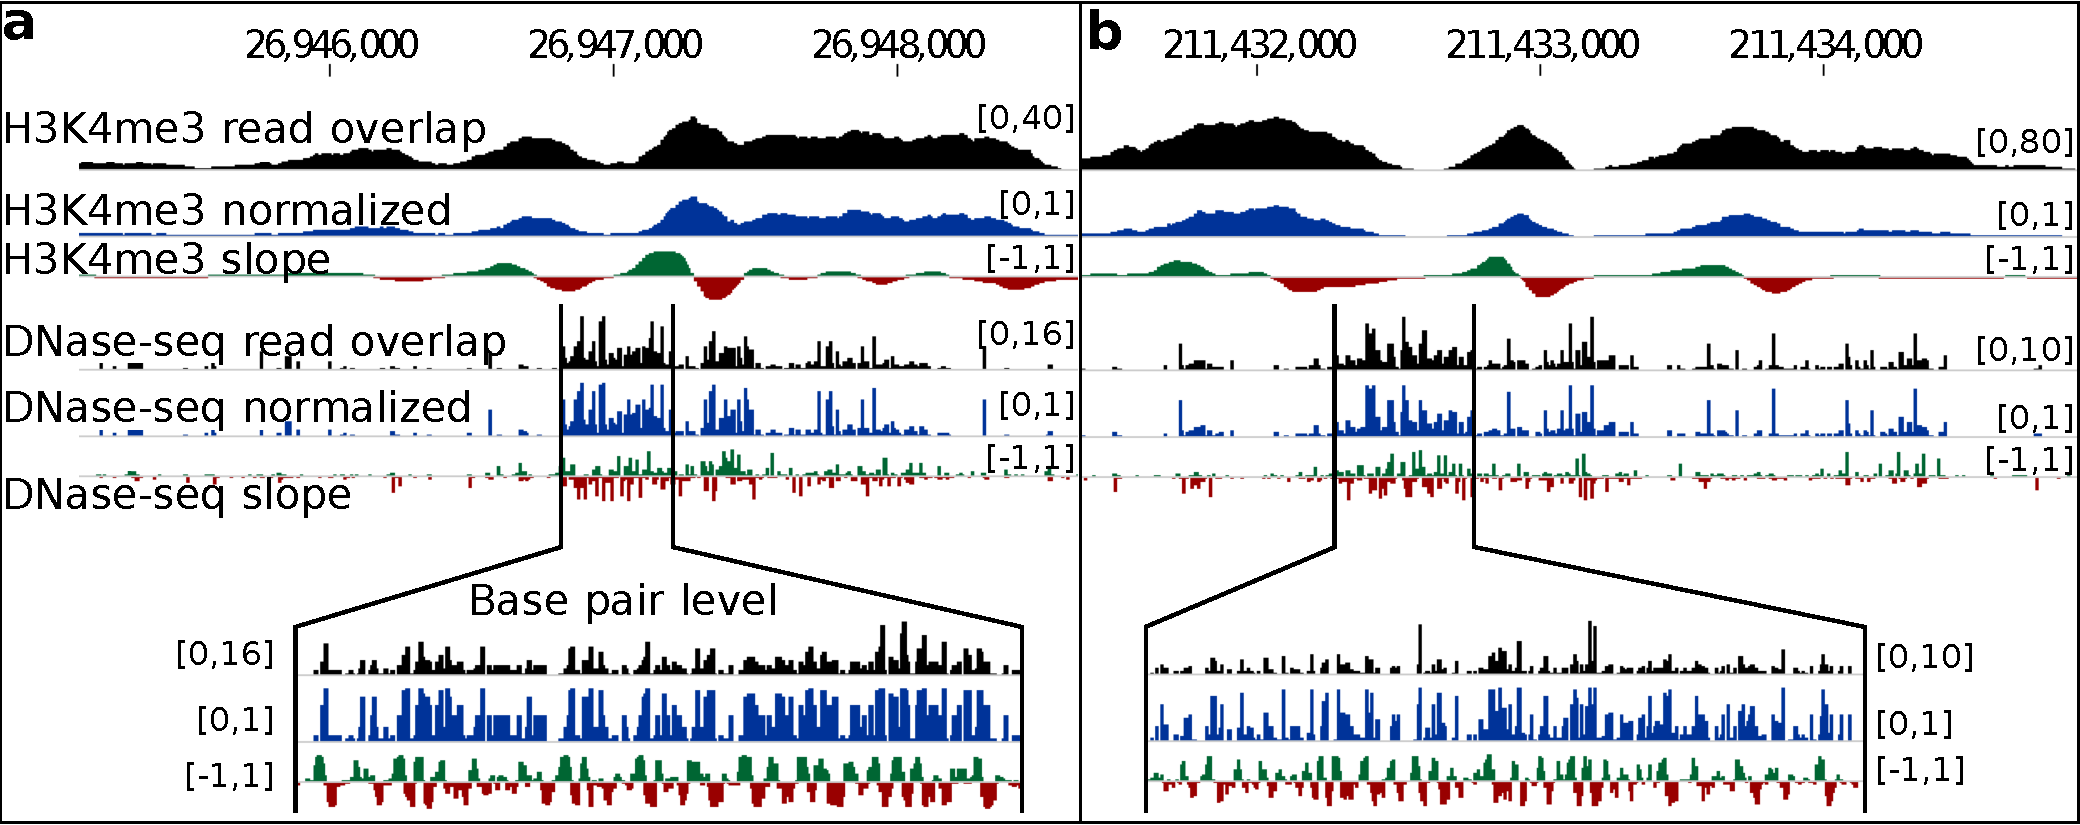
\includegraphics[width=0.99\textwidth]{gusmao_normslope}
\caption[Genomic signal processing examples]{\textbf{Genomic signal processing examples.} Examples of histone modification H3K4me3 ChIP-seq and DNase-seq signals before treatment (Counts; in black), normalized (Normalized; in blue) and after Savitzky-Goaly smoothing and differentiation (Slope; positive values in green and negative values in red). In this figure we show examples for two different regions within human chromosome~1.}
\label{fig:gusmao_normslope}
\end{figure}









%%%%%%%%%%%%%%%%%%%%%%%%%%%%%%%%%%%%%%%%%%%%%%%%%%%%%%%%%%%%%%%%%%%%%
% Section: HINT Training and Application
%%%%%%%%%%%%%%%%%%%%%%%%%%%%%%%%%%%%%%%%%%%%%%%%%%%%%%%%%%%%%%%%%%%%%
\section{HINT Training and Application}
\label{sec:hint.training.application}

% Introduction
As described in Section~\ref{sec:computational.footprinting.hmm} our computational footprinting method -- termed HINT (HMM-based identification of TF footprints) -- relies on the segmentation of the genome using hidden Markov models to process normalized and/or slope signals of DNase-seq and/or histone modification ChIP-seq genomic signals. Such segmentation task is performed on the light of the grammar of active transcription factor binding sites described in Section~\ref{sec:grammar.tfbs}. As depicted in Figure~\ref{fig:gusmao_method_pipeline}c--g we have devised a number of different HMM topologies, which takes different numbers of input signals and address particularities of the TFBS patterns on the experimental chromatin dynamics data. Here, we provide experimental details on how HINT is trained (Section~\ref{sec:hint.training}) and applied on the genome (Section~\ref{sec:hint.application}).

%%%%%%%%%%%%%%%%%%%%%%%%%%%%%%%%%%%%%%%%%%%%%%%%%%%%%%%%%%%%%%%%%%%%%
% Section: HINT Training
%%%%%%%%%%%%%%%%%%%%%%%%%%%%%%%%%%%%%%%%%%%%%%%%%%%%%%%%%%%%%%%%%%%%%
\subsection{HINT Training}
\label{sec:hint.training}

% Manual annotation - introduction
We train the HMM models in a supervised manner. Briefly, a manual annotation is created for each cell type, histone modification and HMM topology (Figure~\ref{fig:gusmao_method_pipeline}c--g) based on the DNase-seq and histone modification ChIP-seq data.

% Manual annotation - region selection
We selected a $10,000$ bp region (with genomic coordinates $211,428,000--211,438,000$ in human chromosome~1) around the promoter of the gene RCOR3 and performed a cell-specific manual annotation, in which each genomic position is assigned with a state from our HMM topology. This promoter-proximal regulatory region annotated with HMM states was used to train the models which use histone modifications H3K4me3, H3K9ac, H3K27ac and H2A.Z. As the histone modification H3K4me1 is known to be associated to distal regulatory regions, we have additionally annotated an enhancer region (with genomic coordinates $26,942,000--26,952,000$ in human chromosome~1). The selection of these regions was made randomly, but we checked ENCODE~\cite{encode2012} tracks for evidence that the gene RCOR3 was expressed in all cell types analyzed and that the enhancer region was far ($>100$ kb) from known genes and expressed regions but associated with the expression of the closest gene's transcription start site.

% Manual annotation - process
In order to help the annotation of the footprints, motif-predicted binding sites (MPBSs) obtained by applying motif matching with all PFMs from Jaspar~\cite{mathelier2014}, Uniprobe~\cite{robasky2011} and Transfac~\cite{matys2006} PFM repositories were detected inside the training regions (the details on the identification of MPBSs can be found in Section~\ref{sec:motif.predicted.binding.sites}). We consider ``real'' footprints all the DNase-seq signal depleted regions between two DNase-seq peaks that overlap a MPBS. For the histone-only HMM topology, we considered as footprints all the DHSs within these regions, obtained as described in Section~\ref{sec:dnaseseq.enriched.regions}. We trained five HMMs per cell type, one for each histone modification (H3K4me3, H3K9ac, H3K29ac and H2A.Z with the promoter-proximal regulatory region and H3K4me1 with the distal regulatory region). In the case of the DNase-only HMM, only one HMM was trained for each cell type. Such training was performed in the promoter-proximal region. The regions used for training were excluded from all further predictions.

% Training
In possession of the manually annotated regions for each cell type, histone modification and HMM topology, all HMMs were trained using the maximum-likelihood process described in Section~\ref{sec:hmm.training}.

% Example of HMM parameters - transition
Here we show an example of a complete set of HMM parameters, regarding the model trained with DNase-seq $+$ H3K4me3 using data from the H1-hESC cell. The Table~\ref{tab:hmmtrans} represents the transition matrix. Each number represents the probability of performing a transition from the HMM state in the first column of the entry's row to the HMM state in the first row of the entry's column. In the transition matrix we are able to observe that only the self-transitions and the transitions allowed by our model topology Figure~\ref{fig:gusmao_method_pipeline}c have a non-zero probability. The transition matrix is the structure that directly defines our HMM topology.

% Example of HMM parameters - emission mean
The Table~\ref{tab:hmmmean} exhibits the emission distribution mean values. It contains the mean in which each signal type (represented in the columns) assumes at each state (represented in the rows). A closer look into these vectors of means for each state and signal shows the grammar of active TFBS in a numerical form. The states {\tt BACK} and {\tt FOOTPRINT} have low absolute means for all signal types. {\tt UP}, {\tt TOP} and {\tt DOWN} states have, respectively, high positive, close to zero and low negative slope signals. Such emission parameters models the signal magnitude of the active TFBS grammar. We are able to model both magnitude and shape of the signals when we consider the transition probabilities and the mean part of the emission probability distributions.

% Example of HMM parameters - emission covariance matrix
Moreover, the Table~\ref{tab:hmmcov} shows all covariance matrices from the emission distributions. The full covariance matrix is depicted for each state, in which rows and columns are sorted by the input signals: DNase normalized, DNase slope, H3K4me3 normalized and H3K4me3 slope. The covariance matrix component of the emission probability distributions reflect the relationship between our signals in our multivariate model. For instance, it is interesting to observe a negative value ($-0.0053$) at the DNase level {\tt UP} state (UP(D) in the table) on the covariance matrix corresponding to the normalized DNase-seq \emph{versus} the normalized histone modification ChIP-seq signal. Such data behaviour is in line with the observed grammar of TFBSs, where the DNase-seq signal generally start to increase at the decrease of the histone modification ChIP-seq signal. Finally, when we consider all HMM parameters, we are able to model the magnitude, shape and relationship between the chromatin dynamics signals.

\begin{table}[t]
\footnotesize
\begin{center}
\caption{Transition probabilities of the HMM trained with H3K4me3 using H1-hESC data. Transitions are specified from the states in the rows to the states in the columns. Histone level states are denoted with `(H)' and DNase level states with `(D)'. The {\tt FOOTPRINT} state is abreviated as `FP'.}
\label{tab:hmmtrans}
    \renewcommand{\arraystretch}{1.2}
    \begin{tabular}{ lllllllll }
        \hline
        & \textbf{BACK} & \textbf{UP (H)} & \textbf{TOP (H)} & \textbf{DOWN (H)} & \textbf{UP (D)}
        & \textbf{TOP (D)} & \textbf{DOWN (D)} & \textbf{FP} \\
        \textbf{BACK}     & 0.9997 & 0.0003 & 0.0    & 0.0    & 0.0    & 0.0    & 0.0   & 0.0    \\
        \textbf{UP (H)}   & 0.0    & 0.9915 & 0.0085 & 0.0    & 0.0    & 0.0    & 0.0   & 0.0    \\
        \textbf{TOP (H)}  & 0.0    & 0.0    & 0.9901 & 0.0099 & 0.0    & 0.0    & 0.0   & 0.0    \\
        \textbf{DOWN (H)} & 0.0057 & 0.0    & 0.0    & 0.9861 & 0.0082 & 0.0    & 0.0   & 0.0    \\
        \textbf{UP (D)}   & 0.0    & 0.0    & 0.0    & 0.0    & 0.6515 & 0.3485 & 0.0   & 0.0    \\
        \textbf{TOP (D)}  & 0.0    & 0.0    & 0.0    & 0.0    & 0.0    & 0.783  & 0.217 & 0.0    \\
        \textbf{DOWN (D)} & 0.0    & 0.0339 & 0.0    & 0.0    & 0.0    & 0.0    & 0.577 & 0.3891 \\
        \textbf{FP}       & 0.0    & 0.0    & 0.0    & 0.0    & 0.0564 & 0.0    & 0.0   & 0.9436 \\
        \hline
    \end{tabular}
\end{center}
\end{table}

\begin{table}[t]
\footnotesize
\begin{center}
\caption{Signals' mean values for each state of the HMM trained with H3K4me3 using H1-hESC data. Histone level states are denoted with `(H)' and DNase level states with `(D)'. The {\tt FOOTPRINT} state is abreviated as `FP'.}
\label{tab:hmmmean}
    \renewcommand{\arraystretch}{1.2}
    \begin{tabular}{ lllll }
        \hline
        & \textbf{DNase norm.} & \textbf{DNase slope} & \textbf{Histone norm.} & \textbf{Histone slope} \\
        \textbf{BACK}     & 0.0045 & -0.0002 & 0.0441 & 0.0007  \\
        \textbf{UP (H)}   & 0.0501 & 0.0043  & 0.1983 & 0.2995  \\
        \textbf{TOP (H)}  & 0.0445 & -0.0075 & 0.4693 & 0.0158  \\
        \textbf{DOWN (H)} & 0.0636 & 0.0003  & 0.2309 & -0.4237 \\
        \textbf{UP (D)}   & 0.1537 & 0.6343  & 0.0894 & -0.0647 \\
        \textbf{TOP (D)}  & 0.4244 & 0.0059  & 0.1091 & -0.0735 \\
        \textbf{DOWN (D)} & 0.1578 & -0.6562 & 0.0816 & -0.0434 \\
        \textbf{FP}       & 0.0902 & -0.0162 & 0.1009 & -0.0436 \\
        \hline
    \end{tabular}
\end{center}
\end{table}

\begin{table}[t]
\footnotesize
\begin{center}
\caption{Covariance matrices for each state of the HMM trained with H3K4me3 using H1-hESC data. Within each state's matrix, lines and rows are sorted by signal type as DNase normalized, DNase slope, H3K4me3 normalized and H3K4me3 slope. Histone level states are denoted with `(H)' and DNase level states with `(D)'. The {\tt FOOTPRINT} state is abreviated as `FP'.}
\label{tab:hmmcov}
    \renewcommand{\arraystretch}{1.2}
    \begin{tabular}{>{\centering\arraybackslash} m{0.2cm}
                    >{\centering\arraybackslash} m{1.2cm}
                    >{\centering\arraybackslash} m{1.2cm}
                    >{\centering\arraybackslash} m{1.2cm}
                    >{\centering\arraybackslash} m{1.2cm}|
                    >{\centering\arraybackslash} m{0.2cm}
                    >{\centering\arraybackslash} m{1.2cm}
                    >{\centering\arraybackslash} m{1.2cm}
                    >{\centering\arraybackslash} m{1.2cm}
                    >{\centering\arraybackslash} m{1.2cm} }
        \hline
        \multirow{4}{*}{\rotatebox[origin=c]{90}{\textbf{BACK}}}
        & 0.0025  & -0.0001 & 0.0001 & 0.0    &
        \multirow{4}{*}{\rotatebox[origin=c]{90}{\textbf{UP (H)}}}
        & 0.0222  & 0.0001  & 0.003  & 0.0057 \\
        & -0.0001 & 0.0025  & 0.0    & 0.0    &
        & 0.0001  & 0.0155  & 0.0006 & 0.0005 \\
        & 0.0001  & 0.0     & 0.0047 & 0.0    &
        & 0.003   & 0.0006  & 0.0101 & 0.0105 \\
        & 0.0     & 0.0     & 0.0    & 0.0019 &
        & 0.0057  & 0.0005  & 0.0105 & 0.0341 \\
        \hline
        \multirow{4}{*}{\rotatebox[origin=c]{90}{\textbf{TOP (H)}}}
        & 0.0216  & 0.0003  & -0.0009 & 0.0014  &
        \multirow{4}{*}{\rotatebox[origin=c]{90}{\textbf{DOWN (H)}}}
        & 0.0239  & 0.0001  & -0.0033 & -0.0002 \\
        & 0.0003  & 0.0196  & 0.0005  & 0.0003  &
        & 0.0001  & 0.009   & 0.0002  & -0.0006 \\
        & -0.0009 & 0.0005  & 0.0047  & -0.001  &
        & -0.0033 & 0.0002  & 0.0156  & -0.0095 \\
        & 0.0014  & 0.0003  & -0.001  & 0.0193  &
        & -0.0002 & -0.0006 & -0.0095 & 0.0313  \\
        \hline
        \multirow{4}{*}{\rotatebox[origin=c]{90}{\textbf{UP (D)}}}
        & 0.0705  & 0.0246  & -0.0053 & 0.0025  &
        \multirow{4}{*}{\rotatebox[origin=c]{90}{\textbf{TOP (D)}}}
        & 0.1559  & -0.002  & -0.0079 & 0.0052  \\
        & 0.0246  & 0.0714  & -0.0038 & -0.0015 &
        & -0.002  & 0.0384  & -0.0008 & 0.0021  \\
        & -0.0053 & -0.0038 & 0.0045  & -0.0056 &
        & -0.0079 & -0.0008 & 0.007   & -0.0096 \\
        & 0.0025  & -0.0015 & -0.0056 & 0.0125  &
        & 0.0052  & 0.0021  & -0.0096 & 0.0184  \\
        \hline
        \multirow{4}{*}{\rotatebox[origin=c]{90}{\textbf{DOWN (D)}}}
        & 0.0687  & -0.011  & -0.0048 & 0.004   &
        \multirow{4}{*}{\rotatebox[origin=c]{90}{\textbf{FP}}}
        & 0.0358  & -0.0019 & -0.0025 & 0.0007  \\
        & -0.011  & 0.055   & 0.0039  & -0.0    &
        & -0.0019 & 0.0225  & 0.0001  & 0.0002  \\
        & -0.0048 & 0.0039  & 0.0039  & -0.0044 &
        & -0.0025 & 0.0001  & 0.0068  & -0.0069 \\
        & 0.004   & -0.0    & -0.0044 & 0.0109  &
        & 0.0007  & 0.0002  & -0.0069 & 0.0121  \\
        \hline
    \end{tabular}
\end{center}
\end{table}


%%%%%%%%%%%%%%%%%%%%%%%%%%%%%%%%%%%%%%%%%%%%%%%%%%%%%%%%%%%%%%%%%%%%%
% Section: HINT Application
%%%%%%%%%%%%%%%%%%%%%%%%%%%%%%%%%%%%%%%%%%%%%%%%%%%%%%%%%%%%%%%%%%%%%
\subsection{HINT Application}
\label{sec:hint.application}

% Selection of genomic regions
To reduce the dimensionality of the data, we first identified the enriched regions on the DNase-seq and histone modification ChIP-seq data (Section~\ref{sec:enriched.regions}). In the DNase + histone HMM topologies (Figure~\ref{fig:gusmao_method_pipeline}c--e), we have extended these enriched regions by $5,000$ bp on each side and merged the resulting regions. These are the regions in which we are going to apply our HMM models. In the DNase-only (Figure~\ref{fig:gusmao_method_pipeline}f) and histone-only HMM (Figure~\ref{fig:gusmao_method_pipeline}g) the extension process is the same, however, using only the DHSs and enriched histone modification peaks, respectively. This step keeps only $3-6\%$ of the genome with DNase-seq or histone modification ChIP-seq evidence for a given cell type (see Supplementary Table~\ref{tab:coverage}).

% HINT application
Given the trained HMM models (Section~\ref{sec:hint.training}), we identify footprints using both approaches described in Section~\ref{sec:hmm.decoding}: (1) using the Viterbi algorithm and (2) using the posterior probability decoding algorithms. This process generates a set of footprints for every model trained and applied and for both decoding algorithms. Each set of footprints are post-processed as described in Section~\ref{sec:footprint.postprocessing}. In the post-processing step, we select the footprint extension ($\rho$) as $5$ bp. Such extension is not high enough to impair the resolution of our predicted footprints. Such footprints represent our predicted active transcription factor binding sites.


% TODO ADD FOOTPRINT EXTENSION HERE












%%%%%%%%%%%%%%%%%%%%%%%%%%%%%%%%%%%%%%%%%%%%%%%%%%%%%%%%%%%%%%%%%%%%%
% Section: Competing Methods
%%%%%%%%%%%%%%%%%%%%%%%%%%%%%%%%%%%%%%%%%%%%%%%%%%%%%%%%%%%%%%%%%%%%%
\section{Competing Methods}
\label{sec:competing.methods}

% Introduction
In this section we present the full descpription of the parameterization and execution of competing methods. The competing methods are categorized as segmentation methods (Neph~\cite{neph2012a}, Boyle~\cite{boyle2011}, Wellington~\cite{piper2013} and DNase2TF~\cite{sung2014}) and site-centric methods (Centipede~\cite{pique2011}, Cuellar~\cite{cuellar2012}, PIQ~\cite{sherwood2014}, FLR~\cite{yardimci2014} and BinDNase~\cite{kahara2015}). Computational resources necessary for the execution of segmentation and site-centric competing methods are summarized in Supplementary Table~\ref{tab:comp.resource}. The table shows the additional steps that the user needs to perform in order to execute the footprinting method, the total CPU time in hours, the maximum memory used during the execution and the total input storage necessary before the execution of each method. Memory consumption and space requirements of all methods are compatible to a high end desktop. Segmentation based methods, which require a execution per cell, are 4 to 200 times faster than the site-centric methods, which require an execution per cell and TF combination. It is important to notice that PIQ is the only site-centric method, which only requires a single exection per cell. The execution of BinDNase and Centipede were particularly time consuming (1 week computing on a 40 core server).

% Baseline methods
In addition to the published segmentation and site-centric methods, we also tested a few baseline methods. The rationale behind these methods is that they are simple in nature and serve as control experiments. The site-centric baseline methods (Section~\ref{sec:sitecentric.baseline.methods}) consists on ranking motif-predicted binding sites (defined in Section~\ref{sec:motif.predicted.binding.sites}) based on footprint quality scores. In addition to these baseline methods we devised a signal processing filter method as a segmentation baseline method (Section~\ref{sec:signal.processing.filters}). All the baseline methods use only DNase-seq data.

% Computational resources to execute methods
\begin{table}[h]
\begin{center}
\caption[Summary of computational resources]{\textbf{Summary of computational resources.} The computational resources were evaluated on 88 TFs binding on cell types H1-hESC (DU) and K562 (DU).} 
\label{tab:comp.resource}
\renewcommand{\arraystretch}{1.2}
\begin{tabularx}{\textwidth}{ lrrrrr }
\hline
Method & Additional Steps & CPU time (hours) & Max. Memory (GB) & Input Storage (GB) \\
\hline
BinDNase & 1,2,4 & 7034 & 8 & 95.7 \\
Boyle & NA$^*$ & NA$^*$ & NA$^*$ & NA$^*$ \\
Centipede & 1,2,4 & 7100 & 8 & 157.7 \\
Cuellar & 1,2,4 & 575 & 32 & 25.4 \\
DNase2TF & 3 & 31 & 32 & 29.3 \\
FLR & 2,4 & 870 & 16 & 43.1 \\
HINT & 3 & 56 & 4 & 17.7 \\
Neph & 3 & 47 & 4 & 14.6 \\
PIQ & - & 386 & 32 & 18.7 \\
Wellington & 3 & 117 & 16 & 14.6 \\
\hline
\multicolumn{6}{l}{$^1$ Requires extra input file processing.} \\
\multicolumn{6}{l}{$^2$ Requires extra motif matching (Section~\ref{sec:motif.predicted.binding.sites}).} \\
\multicolumn{6}{l}{$^3$ Requires extra DNase-seq peak calling (DHSs).} \\
\multicolumn{6}{l}{$^4$ Requires execution of method for each TF.} \\
\multicolumn{6}{l}{$^*$ Implementation not available.} \\
\end{tabularx}
\end{center}
\end{table}

%%%%%%%%%%%%%%%%%%%%%%%%%%%%%%%%%%%%%%%%%%%%%%%%%%%%%%%%%%%%%%%%%%%%%
% Section: Neph Method
%%%%%%%%%%%%%%%%%%%%%%%%%%%%%%%%%%%%%%%%%%%%%%%%%%%%%%%%%%%%%%%%%%%%%
\subsection{Neph Method}
\label{sec:neph}

We obtained the footprint predictions for cell type K562 (DU) in \url{ftp://ftp.ebi.ac.uk/pub/databases/ensembl/encode/supplementary/integration_data_jan2011/byDataType/footprints/jan2011/all.footprints.gz}. As predictions were not available for other DNase-seq experiments, we obtained the scripts and parameterization through Neph et al.~\cite{neph2012a} footprinting method code repository at \url{https://github.com/StamLab/footprinting2012}. Briefly, we used the DNase I raw signal as input with the parameters from the original publication: flanking component length varied between $3$--$10$ bp and central footprint region length varied between $6$--$40$ bp. Afterwards, the footprints were filtered by an FDR of $1\%$, which was estimated based on the FS distribution in each cell type~\cite{neph2012a}. Finally, we consider only predictions that occurred within DNase-seq hotspots, evaluated using the method first described in Sabo et al.~\cite{sabo2004b}. We obtained all hotspots generated by Stamatoyannopoulous' lab in ENCODE for cell types GM12878 (wgEncodeEH000492; GSM736496 and GSM736620), H1-hESC (wgEncodeEH000496; GSM736582) and K562 (wgEncodeEH000484; GSM736629 and GSM736566). We will refer to this framework as ``Neph''.

%%%%%%%%%%%%%%%%%%%%%%%%%%%%%%%%%%%%%%%%%%%%%%%%%%%%%%%%%%%%%%%%%%%%%
% Section: Boyle Method
%%%%%%%%%%%%%%%%%%%%%%%%%%%%%%%%%%%%%%%%%%%%%%%%%%%%%%%%%%%%%%%%%%%%%
\subsection{Boyle Method}
\label{sec:boyle}

Since no source code or software is provided, we used footprint predictions from Boyle et al.~\cite{boyle2011} available at~\url{http://fureylab.web.unc.edu/datasets/footprints/}. We will refer to this method as ``Boyle''.

%%%%%%%%%%%%%%%%%%%%%%%%%%%%%%%%%%%%%%%%%%%%%%%%%%%%%%%%%%%%%%%%%%%%%
% Section: Centipede
%%%%%%%%%%%%%%%%%%%%%%%%%%%%%%%%%%%%%%%%%%%%%%%%%%%%%%%%%%%%%%%%%%%%%
\subsection{Centipede}
\label{sec:centipede}

Centipede software was obtained at~\url{http://centipede.uchicago.edu/} and executed to generate posterior probabilities of regions being bound by TFs. The experimental and genomic data used include DNase-seq, position weight matrix (PWM) bit-score, sequence conservation and distance to the nearest transcription start site (TSS). The experimental data input was generated by fetching the raw DNase-seq signal surrounding a 200 bp window centered on each MPBS. Additionally, we used conservation score, distance to the nearest TSS and the PWM bit-score to create the required prior probabilities. These additional genomic data were obtained from PhastCons conservation score (placental mammals on the 46-way multiple alignment)~\cite{siepel2005} and Ensembl gene annotation from ENCODE~\cite{hubbard2002}.

All parameters were set to their default values, with exception of the level of shrinkage of multinomial parameters ($L$) and the level of shrinkage of negative binomial parameters ($N$). We observed that Centipede is very sensitive to these parameters and we performed an extensive computational analysis to estimate these parameters. It was found that the best parameterization is: $L=0.75$ and $N=0$ for H1-hESC cell; and $L=0.75$ and $N=0.25$ for K562 cell. The full description on the parameter estimation can be found in Section~\ref{xxx}.

%%%%%%%%%%%%%%%%%%%%%%%%%%%%%%%%%%%%%%%%%%%%%%%%%%%%%%%%%%%%%%%%%%%%%
% Section: Cuellar Method
%%%%%%%%%%%%%%%%%%%%%%%%%%%%%%%%%%%%%%%%%%%%%%%%%%%%%%%%%%%%%%%%%%%%%
\subsection{Cuellar Method}
\label{sec:cuellar}

We applied this method as described in Cuellar-Partida et al.~\cite{cuellar2012}. We created a smoothed DNase-seq input signal by evaluating the number of DNase-seq cleavage based on a $150$ bp window with $20$ bp steps. We obtained their scripts at~\url{http://tlbailey.bitbucket.org/supplementary_data/Cuellar2011/} and created priors using the smoothed version of the DNase-seq signal. As suggested by the authors, the priors were submitted to the program FIMO~\cite{grant2011} to obtain the predictions. We will refer to this method as ``Cuellar''.

We also observed that the predictions are very sensitive to the $p$-value cutoff threshold from the program FIMO. Therefore, we performed an extensive computational analysis to estimate this parameter. It was found that the best cutoff threshold is at $10^{-5}$. The full description on the parameter estimation can be found in Section~\ref{xxx}.

%%%%%%%%%%%%%%%%%%%%%%%%%%%%%%%%%%%%%%%%%%%%%%%%%%%%%%%%%%%%%%%%%%%%%
% Section: Wellington
%%%%%%%%%%%%%%%%%%%%%%%%%%%%%%%%%%%%%%%%%%%%%%%%%%%%%%%%%%%%%%%%%%%%%
\subsection{Wellington}
\label{sec:wellington}

We have obtained Wellington's source code in ~\url{http://jpiper.github.com/pyDNase} and executed it with default parameters. Briefly, we used a footprint FDR cutoff of $-30$, footprint sizes varying between $6$ and $40$ with $1$ bp steps and shoulder size (flanking regions) of $35$ bp.

%%%%%%%%%%%%%%%%%%%%%%%%%%%%%%%%%%%%%%%%%%%%%%%%%%%%%%%%%%%%%%%%%%%%%
% Section: Protein Interaction Quantification (PIQ)
%%%%%%%%%%%%%%%%%%%%%%%%%%%%%%%%%%%%%%%%%%%%%%%%%%%%%%%%%%%%%%%%%%%%%
\subsection{Protein Interaction Quantification (PIQ)}
\label{sec:piq}

We obtained PIQ implementation in~\url{http://piq.csail.mit.edu} and executed it with default parameters, which can be found in the script {\emph common.r}. Briefly, MPBSs were generated with the script {\emph pwmmatch.exact.r}. The DNase-seq signal was created using the script {\emph bam2rdata.r}. And the footprints were detected with the script {\emph pertf.r}.

%%%%%%%%%%%%%%%%%%%%%%%%%%%%%%%%%%%%%%%%%%%%%%%%%%%%%%%%%%%%%%%%%%%%%
% Section: Footprint Mixture (FLR)
%%%%%%%%%%%%%%%%%%%%%%%%%%%%%%%%%%%%%%%%%%%%%%%%%%%%%%%%%%%%%%%%%%%%%
\subsection{Footprint Mixture (FLR)}
\label{sec:flr}

Method implementation was obtained in~\url{https://ohlerlab.mdc-berlin.de/software/FootprintMixture_109/}. We executed the method using the $6$-mer cleavage bias frequencies for initialization of the background models. The width of the window surrounding the TFBSs ({\emph PadLen}) was set to the default value of $25$ bp. Also, we use the expectation maximization to re-estimate background during training (argument {\emph Fixed} set to FALSE). We will refer to this method as ``FLR''.

%%%%%%%%%%%%%%%%%%%%%%%%%%%%%%%%%%%%%%%%%%%%%%%%%%%%%%%%%%%%%%%%%%%%%
% Section: DNase2TF
%%%%%%%%%%%%%%%%%%%%%%%%%%%%%%%%%%%%%%%%%%%%%%%%%%%%%%%%%%%%%%%%%%%%%
\subsection{DNase2TF}
\label{sec:dnase2tf}

We obtained source code from~\url{http://sourceforge.net/projects/dnase2tfr/} and executed DNase2TF with a $4$-mer cleavage bias correction. Other parameters were set to their default values: {\emph minw} $= 6$, {\emph maxw} $= 30$, {\emph z\_threshold} $= -2$ and {\emph FDR} $= 10^{-3}$.

%%%%%%%%%%%%%%%%%%%%%%%%%%%%%%%%%%%%%%%%%%%%%%%%%%%%%%%%%%%%%%%%%%%%%
% Section: BinDNase
%%%%%%%%%%%%%%%%%%%%%%%%%%%%%%%%%%%%%%%%%%%%%%%%%%%%%%%%%%%%%%%%%%%%%
\subsection{BinDNase}
\label{sec:bindnase}

As a supervised approach, the method requires positive and negative examples, which can be obtained from TF ChIP-seq data (see Section~\ref{sec:chipseq.evaluation}). We have used DNase-seq data around MPBSs on chromosome 1 for training. These MPBSs were subsequently removed from the evaluation procedure. Note that this is the only method evaluated here which requires TF ChIP-seq examples for training. We also point the fact that BinDNase did not successfully executed for $19$ TFs of our evaluation data set (POU5F1, REST, RFX5, SP1, SP2, SRF, TCF12 and ZNF143 binding in H1-hESC; ARID3A, CTCF, IRF1, MEF2A, PU1, REST, RFX5, SP1, SP2, STAT2 and ZNF263 binding in K562) given our maximum running time criteria (three weeks). Method implementation was obtained at~\url{http://research.ics.aalto.fi/csb/software/bindnase/} and required/provided no parameter selection.

%%%%%%%%%%%%%%%%%%%%%%%%%%%%%%%%%%%%%%%%%%%%%%%%%%%%%%%%%%%%%%%%%%%%%
% Section: Site-centric Baseline Methods
%%%%%%%%%%%%%%%%%%%%%%%%%%%%%%%%%%%%%%%%%%%%%%%%%%%%%%%%%%%%%%%%%%%%%
\subsection{Site-centric Baseline Methods}
\label{sec:sitecentric.baseline.methods}

% Introduction
The site-centric baseline methods consist on ranking the motif-predicted binding sites for a particular transcription factor based on a quality metric. The motif-predicted binding sites can be seen as a set of genomic regions $R = \{ {r}_{1}, \cdots, {r}_{m} \}$ in which each ${r}_{i} = [u,v]$ represents a binding site prediction (genomic region from $u$ to $v$) based solely on the DNA sequence and the protein's binding affinity to that DNA sequence. The motif-predicted binding sites are obtained through the string-matching process called motif matching, which is described in Section~\ref{sec:motif.predicted.binding.sites}.

% PWM-Rank
\subsubsection{PWM-Rank}
\label{sec:pwm.rank}

% PWM-Rank
The PWM-Rank is a baseline method which consists on ranking motif-predicted binding sites based on their motif match bit-score. Such metric is obtained directly from the motif matching procedure (see Section~\ref{sec:motif.predicted.binding.sites}). The terminology ``PWM'' stands for ``position weight matrix'', which is the binding affinity structure that is used to evaluate the bit-scores in the motif matching procedure. This method can be considered the ``absolute control'', since it does not use any experimental evidence of chromatin structure to detect active transcription factor binding sites. Consequently, the results for the PWM-Rank method are the same for all the cell's in the same organism, since they share the same DNA sequence.

% TC-Rank
\subsubsection{TC-Rank}
\label{sec:tc.rank}

% TC-Rank
The TC-Rank method consists on ranking the motif-predicted binding sites based on the tag count (TC) within their vicinity. The method's rationale is that the more tag counts in the vicinity of a motif-predicted binding site, the more likely it is to be inside an open-chromatin region and therefore be an active transcription factor binding site. In this thesis we use the most predominant window size for the tag count calculation, which is $200$ bp in total~\cite{cuellar2012,he2014}. Let $R = \{ {r}_{1}, \cdots, {r}_{m} \}$ be a set of motif-predicted binding sites for a particular transcription factor and $\mathbf{x}$ the raw DNase-seq signal, the tag count score for the motif-predicted binding site ${r}_{i} = [u,v]$ can be written as
\begin{align}
\text{TC}_{{r}_{i}} = \sum_{j=\frac{(u+v)}{2} - 100}^{\frac{(u+v)}{2} + 100} {x}_{j}.
\label{eq:tc}
\end{align}

% FS-Rank
\subsubsection{FS-Rank}
\label{sec:fs.rank}

% FS-Rank
The FS-Rank method consists on ranking the motif-predicted binding sites based on the footprint score (FS) metric, which was used in previous works~\cite{neph2012a,he2014} as a quality score to rank footprints predictions. The method's rationale is that a motif-predicted binding site with few DNase I cleavage within the binding site region in comparison to its flanking regions corresponds to the pattern described as the grammar of active transcription factor binding sites and therefore is more likely to be an active transcription factor binding site. Let $R = \{ {r}_{1}, \cdots, {r}_{m} \}$ be a set of motif-predicted binding sites for a particular transcription factor and $\mathbf{x}$ the raw DNase-seq signal, the footprint score for the motif-predicted binding site ${r}_{i} = [u,v]$ can be written as
\begin{align}
\text{FS}_{{r}_{i}} = -\left(\frac{{n}_{C}+1}{{n}_{R}+1} + \frac{{n}_{C}+1}{{n}_{L}+1}\right),
\label{eq:fs1}
\end{align}
where ${n}_{C}$, ${n}_{L}$ and ${n}_{R}$ are the number of DNase I cleavage hits within the motif-predicted binding site, in the left (upstream) region of the motif-predicted binding site and in the right (downstream) region of the motif-predicted binding site. These values can be written as
\begin{align}
{n}_{C} &= \sum_{j=u}^{v} {x}_{j}, &
{n}_{R} &= \sum_{j=v}^{2v-u} {x}_{j}, &
{n}_{L} &= \sum_{j=2u-v}^{u} {x}_{j}.
\label{eq:fs2}
\end{align}

%%%%%%%%%%%%%%%%%%%%%%%%%%%%%%%%%%%%%%%%%%%%%%%%%%%%%%%%%%%%%%%%%%%%%
% Section: Signal Processing Filters
%%%%%%%%%%%%%%%%%%%%%%%%%%%%%%%%%%%%%%%%%%%%%%%%%%%%%%%%%%%%%%%%%%%%%
\subsection{Signal Processing Filters}
\label{sec:signal.processing.filters}

% Introduction
The rationale of using signal processing filters for computational footprinting is to remove inadequate frequencies in order to make the DNase-seq peaks more pronounced and detectable by simpler window-based approaches. The method works as follows. First, filtering techniques are applied to regions enriched with DNase-seq signal (DNase I hypersensitivity regions). Then, we apply a standard deviation-based windowing approach to detect the significant depletions in the data, i.e. the footprint pattern.

% Signal Filtering
\subsubsection{Signal Filtering}
\label{sec:signal.filtering}

% Signal filtering 1
For each genomic region enriched for the selected genomic features, we applied one of these four filtering techniques: (1) the Butterworth filter, (2) the Chebyshev filter, (3) the Elliptic filter and (4) the Bessel filter. These filters differ based on the shape of their frequency response and are defined based on their transfer functions in the following paragraphs.

% Butterworth
\textbf{Butterworth Filter}: The rationale behind the butterworth filter is that an ideal signal processing filter should not only completely reject the unwanted frequencies but should also have uniform sensitivity for the wanted frequencies. Such an ideal filter can not be achieved but it can be shown that successively closer approximations are obtained with increasing numbers of filter elements of the right values. It was shown that a low-pass filter could be designed whose cutoff frequency was normalized to $1$ radian per time unit and whose frequency response (gain) was
\begin{equation}
  \label{eq:butterworth1}
  G_n(\omega) = \sqrt{\frac{1}{{1+\omega^{2n}}}},
\end{equation}
where $ \omega $ is the angular frequency in radians per time unit $ t $ (which corresponds to our genomic coordinates) and $n$ is the number of poles in the filter.

% Chebyshev
\textbf{Chebyshev Filter}: The Chebyshev filter allows for variation near the passband around the cutoff, which allows a much better roll off. Thus, it can accurately remove the unwanted frequencies but at the cost of inaccuracy near the cutoff region for the pass band frequency. More formally, Chebyshev filters have the property that they minimize the error between the idealized and the actual filter characteristic over the range of the filter but with ripples in the passband. There are two possible implementations of the chebyshev filters, termed type I and II. In this work we focus on the type I Chebyshev filter, since it does roll off faster than the type II. Furthermore, the type II require more components, which makes the parameters selection more difficult and more prone to overfitting. The Chebyshev type I transfer function is defined as
\begin{equation}
  \label{eq:chebyshev1}
  G_n(\omega) = \frac{1}{\sqrt{1+{\epsilon^2 {T}_{n}^{2} (\frac{\omega}{\omega_0})}}},
\end{equation}
where $ \omega $ is the angular frequency in radians per time unit $ t $ (which corresponds to our genomic coordinates), $n$ is the number of poles in the filter, $ \epsilon $ is the ripple factor, $ \omega_0 $ is the cutoff frequency and $ T_n $ is a Chebyshev polynomial of the $n^{\text{th}}$-order.

% Elliptic
\textbf{Elliptic Filter}: An elliptic filter is a signal processing filter with equalized ripple behavior in both the passband and the stopband. The amount of ripple in each band is independently adjustable, and no other filter of equal order can have a faster transition in gain between the passband and the stopband, for the given values of ripple (whether the ripple is equalized or not). Alternatively, one may give up the ability to adjust independently the passband and stopband ripple, and instead design a filter which is maximally insensitive to component variations. As the ripple in the stopband approaches zero, the filter becomes a type I Chebyshev filter. As the ripple in the passband approaches zero, the filter becomes a type II Chebyshev filter and finally, as both ripple values approach zero, the filter becomes a Butterworth filter. More formally, the gain of the elliptic filter is given by
\begin{equation}
  \label{eq:elliptic1}
  G_n(\omega)=\frac{1}{\sqrt{1+{ \epsilon^2 R_n^2(\xi,\omega/\omega_0)}}},
\end{equation}
where $ \omega $ is the angular frequency in radians per time unit $ t $ (which corresponds to our genomic coordinates), $n$ is the number of poles in the filter, $ \epsilon $ is the ripple factor, $ \omega_0 $ is the cutoff frequency, $ \xi $ is the selectivity factor and $ R_n $ is the $n^{\text{th}}$-order elliptic rational function.

% Bessel
\textbf{Bessel Filter}: The Bessel filter is a signal processing filter with a maximally flat group/phase delay (maximally linear phase response), which preserves the wave shape of filtered signals in the passband. More formally, the Bessel filter can be characterized as
\begin{equation}
  \label{eq:bessel1}
  G_n(\omega) = \frac{\theta_n(0)}{\theta_n(\omega/\omega_0)},
\end{equation}
where $ \omega $ is the angular frequency in radians per time unit $ t $ (which corresponds to our genomic coordinates), $n$ is the number of poles in the filter, $ \omega_0 $ is the cutoff frequency and $ \theta_n(s) $ is the $n^{\text{th}}$-order reverse Bessel polynomial.

% Signal filtering 2
We observed that the accuracy is impacted by selecting different filter parameters. Therefore, a full parameterization analysis was performed (Section~\ref{xxx}). Within this framework we are able to perform the signal frequency and time-domain transformations. For every filter, we applied the implementations of their high-pass, low-pass and band-stop filters: (1) the high-pass filter removes background noise in the data; (2) the low-pass filter attenuates the peaks in the genomic signal and (3) band-stop filter normalize the signals in order to prepare them for the standard deviation-based footprinting.

% Signal filtering 3
Such three-filter approach is possible given the fact that there is no stability danger since we are not bound by hardware-implementation of the filters. Such implementation provides a significant filtering roll off, which depends only on the parameter selection for each filter type. All filters output real-valued signals which contains negative values. In order to prevent numerical problems on the standard deviation-based footprinting which these negative values might cause, we evaluated the global minimum value and summed the absolute version of this value for all values of the genomic signal.

\subsubsection{Standard Deviation Footprinting}
\label{sec:standard.deviation.footprinting}

% Experimental standard deviation
The second part of the method corresponds to the statistical analysis of the filtered signal to obtain the footprint predictions. First, we measured the average standard deviation within the filtered signal for: (1) a $20$ bp window centered at the beginning of all motif-predicted binding sites (see Section~\ref{sec:motif.predicted.binding.sites}) in the human chromosome~1, (2) a $20$ bp window centered at the ending of all motif-predicted binding sites in the human chromosome~1. We call these values, respectively $ \bar{\alpha} $ and $ \bar{\beta} $. We considered all MPBSs obtained by applying motif matching in cell type K562 and we considered the true MPBS the ones that contained ChIP-seq evidence (see Section~\ref{sec:chipseq.evaluation}). The human chromosome~1 was removed from all subsequent evaluation experiments.

% Standard deviation footprinting
Then, we are able to perform a window-based search within the genomic signal for $ k $ bp regions in which the standard deviation evaluated at a $20$ bp window from the region's start site (and region's end site) does not excede a certain threshold value $ \hat{\alpha} $ (and $ \hat{\beta} $) from the experimentally-evaluated standard deviations $ \bar{\alpha} $ (and $ \bar{\beta} $). Such approach consists on a slightly modified version of the algorithm proposed by Neph et al.~\cite{neph2012a}. Such modifications were performed in order to fit the filtered signals. The standard deviations are evaluated dynamically as the window slides within the selected regions. Finally, we observed that the accuracy is impacted by selecting different values of $ k $, $ \bar{\alpha} $ and $ \bar{\beta} $. Therefore, a full parameterization analysis was performed (Section~\ref{xxx}).









%%%%%%%%%%%%%%%%%%%%%%%%%%%%%%%%%%%%%%%%%%%%%%%%%%%%%%%%%%%%%%%%%%%%%
% Section: Method Evaluation Strategies
%%%%%%%%%%%%%%%%%%%%%%%%%%%%%%%%%%%%%%%%%%%%%%%%%%%%%%%%%%%%%%%%%%%%%
\section{Method Evaluation Strategies}
\label{sec:method.evaluation.strategies}

% Introduction
In this section we discuss the methodology used to evalute the footprint predictions from our method and competing methods. We used two evaluation approaches. The first is based on transcription factor ChIP-seq data (ChIP-seq evaluation) and was generally used in the literature to compare computational footprinting methods~\cite{pique2011,boyle2011,cuellar2012}. Nevertheless, transcription factor ChIP-seq experiments need to be carried out on the very same cells as the DNase-seq or histone modification ChIP-seq experiments in which the footprint predictions are being made and has a few caveats. First, transcription factor ChIP-seq peaks are also observed in indirect binding events~\cite{yardimci2014}. Second, their low spatial resolution makes that false binding sites might be regarded as true binding sites by proximity tthe actual binding site~\cite{cuellar2012,yardimci2014}. Therefore, we devised a second evaluation approach which does not require transcription factor ChIP-seq data. Instead, it is based on gene expression differences from pairs of cells (gene expression evaluation).

% MPBSs
Both evaluation strategies uses motif-predicted binding sites, which are transcription factor binding sites predicted using only DNA sequence information and the DNA sequence affinity that proteins have (see Section~ref{sec:computational.sequence.method}). In this thesis we used the computational sequence-based method termed motif matching (Section~\ref{sec:motif.predicted.binding.sites}). Then we proceed by defining an interval-based algebra, which formalizes a number of functions regarding relations between sets of genomic regions (Section~\ref{sec:interval.based.algebra}). Such definitions are required to further describe the evaluation methodologies based on ChIP-seq (Section~\ref{sec:chipseq.evaluation}) and gene expression (Section~\ref{sec:gene.expression.evaluation}).

%%%%%%%%%%%%%%%%%%%%%%%%%%%%%%%%%%%%%%%%%%%%%%%%%%%%%%%%%%%%%%%%%%%%%
% Section: Motif-Predicted Binding Sites
%%%%%%%%%%%%%%%%%%%%%%%%%%%%%%%%%%%%%%%%%%%%%%%%%%%%%%%%%%%%%%%%%%%%%
\subsection{Motif-Predicted Binding Sites}
\label{sec:motif.predicted.binding.sites}

% Introduction
Motif-predicted binding sites are predictions of transcription factor binding sites made using only the genomic DNA sequence and the proteins' DNA sequence binding addinity. Motif-predicted binding sites can be obtained applying a computational sequence-based method to identify binding sites. In this thesis we use an algorithm termed motif matching. The motif matching algorithm can be divided into two parts. First, we calculate a mathematical representation of the protein DNA sequence binding affinity called position weight matrix (PWM). Then, we scan the genomic DNA sequence using the position weight matrix to find substrings which are more likely to represent binding sites. This scanning process, which can be seen as a martix-vector convolution, is called motif matching.

% Section - Position Weight Matrices
\subsubsection{Position Weight Matrices}

% Introduction
Position weight matrices are mathematical representation of the underlying DNA sequences in which a target protein has binding affinity. Here, we describe how this structure can be created. The Figure~\ref{fig:wasserman_pwm} shows a graphical representation of an example of a position weight matrix.

% PFMs
The first step is to gather experimentally verified biological sequences which are known to be bound by the target transcription factor of interest. There are multiple types of biological experiments which can be performed in order to assess these sequences, including ChIP-seq. Then, a multiple alignment algorithm is applied to these experimentally verified DNA sequences. After that, conserved positions within this multiple alignment are determined and a specific window, that varies from $5$--$25$ bp is estimated to be the start and end position of the binding affinity representation (Figure~\ref{fig:wasserman_pwm}a and~b).

% PFMs
At this point, a matrix termed position frequency matrix (PFM) $\mathbf{X}^{4 \times m}$ (Figure~\ref{fig:wasserman_pwm}c) is created in the following way: each matrix row $i \in D\}$ with $D = \{\text{A},\text{C},\text{G},\text{T}\}$, correspond to each one of the possible four DNA nucleotides; and the each matrix column $ j \in \{1, \cdots, m\} $ correspond to a position within the motif in the multiple aligned DNA sequences. Consequently, $m$ represents the total length of the motif. Each entry $x_{ij}$ of the PFM corresponds to the number of nucleotides of type $ i $ in position $ j $ of the DNA framents' multiple alignment.

% PWMs
From PFMs, we are able to create normalized logarithmic representations termed position weight matrices (PWMs) $\mathbf{W}^{4 \times m}$ (Figure~\ref{fig:wasserman_pwm}d). The most common method to create PWMs consists on the calculation of the corrected probability $ p_{ij} $ of finding the nucleotide $ i $ in the position $ j $, which is given by
\begin{equation}
  \label{eq:pwm1}
  p_{ij} = \frac{ f_{ij} + s(i) }{ m + {\sum\limits _{i^\prime \in D}{ \hspace{-0.0cm} s(i^\prime)}} }, 
\end{equation}
where $ f_{ij} $ is the frequency of base $ i $ at position $ j $ and $ s(i) $ is a pseudocount function. Pseudocounts are small values used to avoid null probabilities. After the evaluation of the corrected probabilities, the entries $ w_{ij} $ of the PWM can be calculated as
\begin{equation}
  \label{eq:pwm2}
  w_{ij} = \log_2 \frac{ p_{ij} }{ b(i) }, 
\end{equation}
where $ b(i) $ is the genomic frequency of nucleotide $ i $ in the genome. The background correction function $b(\cdot)$ is used to correct the PWM for biases regarding the genomic imbalance between the frequencies of the nucleotides.

% Scoring
The PWMs can be used to score any DNA sequence of length $m$ by a summation of the correponding nucleotides between the DNA sequence and the PWM (Figure~\ref{fig:wasserman_pwm}e). Such a score is called the PWM's bit-score.

% Information content
Furthermore, we are able to assess the information content $ \mathbf{l} = \langle{l}_{1}, ..., {l}_{m}\rangle $ of each position $ j $ of the PWM $ \mathbf{W} $ by applying
\begin{equation}
  \label{eq:pwm.ic}
  {l}_{j} = 2 + \sum\limits _{i \in D} p_{ij} \log_{2} p_{ij},
\end{equation}
where the number $2$ is obtained from the total possible information content of the $4$-character alphabet $D$, i.e. $\log_{2}4 = 2$. Based on the total information content for every position of the PWM, we are able to create graphical representations of the binding affinity -- termed logo graphs (Figure~\ref{fig:wasserman_pwm}f) -- by multiplying the corrected probability of a certain nucleotide $i$ at a certain position of the PWM $j$ by the total information content at that position (${l}_{j}$).

% Figure - Position weight matrices (PWMs)
\begin{figure}[h!]
\centering
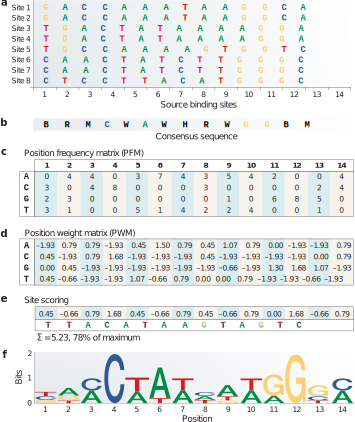
\includegraphics[width=0.7\textwidth]{wasserman_6_pwm}
\caption[Position weight matrices (PWMs)]{\textbf{Position weight matrices (PWMs).}The first step towards building models for predicting transcription factor binding sites involves data collection. To illustrate the process, we use the transcription factor MEF2 as an example. (\textbf{a}) A set of experimentally validated MEF2-binding sites was collected from the literature and aligned. The sequence variability of the collection of binding sites strongly affects the downstream models for predicting additional sites. Note the diversity between the sites; for instance, only $50\%$ of the nucleotides are identical between sites one and eight. (\textbf{b}) Here we show, for illustrative purposes, a consensus sequence model, which is defined by selecting a degeneracy nucleotide symbol for each position (column) in the alignment. For instance, the symbol ``B'' means preference for either nucleotides C, G or T. (\textbf{c}) To more accurately reflect the characteristics at each position, a matrix that contains the number of observed nucleotides at each position is created. For instance, the first column in the alignment consists of no As, three Cs, two Gs and three Ts, therefore resulting in the corresponding first matrix column $\langle 0, 3, 2, 3 \rangle$. (\textbf{d}) The frequency matrix is usually converted to a position weight matrix (PWM) using a the procedure described by Equations~\ref{eq:pwm1},~\ref{eq:pwm2}. (\textbf{e}) Using a matrix model, a quantitative score for any DNA sequence can be generated by summing the values that correspond to the observed nucleotide at each position. This procedure can be repeated for all contiguous sequences in the genome, which consist on the motif matching method, formally described by Equations~\ref{eq:motif.match}--\ref{eq:pwm.cutoff2}. (\textbf{f}) The specificity in each column of the alignment can be measured in terms of information content. A sequence logo scales each nucleotide by the total bits of information multiplied by the relative occurrence of the nucleotide at the position (see Equation~\ref{eq:pwm.ic}). Sequence logos enable fast and intuitive visual assessment of pattern characteristics. \emph{Source: Wasserman et al.}\cite{wasserman2004} (modified to fit thesis format and/or clarify key points).}
\label{fig:wasserman_pwm}
\end{figure}

% Section - Motif Matching
\subsubsection{Motif Matching}

% Motif matching
From a PWM it is possible to evaluate the probability of the particular TF, in which the PWM was created, of binding in the genome. We call this procedure motif matching. For each sequence of nucleotides of length $ m $, a bit-score can be evaluated. There are also many strategies to perform this calculation. The simples one is the summation of all the entries in $ w_{ij} $ matching the nucleotide sequence of length $ m $. More formally, given a sequence of characters $\mathbf{g}$ representing the genome, where $\mathbf{g} = \langle{g}_{1}, ..., {g}_{n}\rangle \forall {g}_{i} \in D$. We are able to define a vector of bit-scores $\mathbf{y} = \langle{y}_{1}, ..., {y}_{n-m}\rangle$ as
\begin{equation}
  \label{eq:motif.match}
  {y}_{i} = \sum_{j=1}^{m} \sum_{k \in D} {\mathbf{1}}(k={g}_{i}){w}_{kj},
\end{equation}
where ${\mathbf{1}}(\cdot)$ is an indicator function. 

% Motif match cutoff threshold
A genome-wide application of a PWM creates bit-scores for every possible contiguous nucleotide sequence of length $ N $ within the genome. Then, several statistical techniques can be used to determine a cutoff threshold to accept particular sequences as being bound by the protein, given the PWM. A well-known statistical procedure is to evaluate a bit-score cutoff that corresponds to the false positive rate (FPR) of the distribution of the bit-scores from all possible $m$-mers~\cite{wilczynski2009}. More formally, let $C = \{\mathbf{c}^{1}, ..., \mathbf{c}^{4^m}\}$ be the set of all $m$-mers constructed by picking $ m $ elements from the set $ D $ with order and repetition, where each $m$-mer $\mathbf{c}^{i} = \langle{c}^{i}_{1}, \cdots, {c}^{i}_{m}\rangle$. Therefore, we are able to evaluate the set $ B = \{ {b}_{1}, \cdots, {b}_{4^m} \} $ of all the possible bit-scores for the PWM $\mathbf{W}$ as
\begin{equation}
  \label{eq:pwm.cutoff1}
  {b}_{i} = \sum_{j=1}^{m} \sum_{k \in D} {\mathbf{1}}(k={c}^{i}_{j}){w}_{kj}.
\end{equation}

% Motif match cutoff threshold
Then, it is easy to find the false discovery rate threshold by finding the $p$-value that corresponds to $ B $ fitted to a certain distribution, say normal
\begin{equation}
  \label{eq:pwm.cutoff2}
  B \sim \mathcal{N}({\mu},{\sigma}^{2}).
\end{equation}

% Set of motif-predicted binding sites
We observed that the $p$-value choice significantly affects many aspects of the evaluation procedure. Therefore we made a careful parameter selection analysis (Section~\ref{xxx}). Finally, the set of motif-predicted binding sites after the application of the false discovery rate cutoff threshold is going to be denoted in this section as $M = \{ {m}_{1}, \cdots, {m}_{l} \}$.

%%%%%%%%%%%%%%%%%%%%%%%%%%%%%%%%%%%%%%%%%%%%%%%%%%%%%%%%%%%%%%%%%%%%%
% Section: Interval-Based Algebra
%%%%%%%%%%%%%%%%%%%%%%%%%%%%%%%%%%%%%%%%%%%%%%%%%%%%%%%%%%%%%%%%%%%%%
\subsection{Interval-Based Algebra}
\label{sec:interval.based.algebra}

% TODO





%%%%%%%%%%%%%%%%%%%%%%%%%%%%%%%%%%%%%%%%%%%%%%%%%%%%%%%%%%%%%%%%%%%%%
% Section: ChIP-seq Evaluation
%%%%%%%%%%%%%%%%%%%%%%%%%%%%%%%%%%%%%%%%%%%%%%%%%%%%%%%%%%%%%%%%%%%%%
\subsection{ChIP-seq Evaluation}
\label{sec:chipseq.evaluation}




%%%%%%%%%%%%%%%%%%%%%%%%%%%%%%%%%%%%%%%%%%%%%%%%%%%%%%%%%%%%%%%%%%%%%
% Section: Gene Expression Evaluation
%%%%%%%%%%%%%%%%%%%%%%%%%%%%%%%%%%%%%%%%%%%%%%%%%%%%%%%%%%%%%%%%%%%%%
\subsection{Gene Expression Evaluation}
\label{sec:gene.expression.evaluation}












%%%%%%%%%%%%%%%%%%%%%%%%%%%%%%%%%%%%%%%%%%%%%%%%%%%%%%%%%%%%%%%%%%%%%
% Section: Statistical Methods
%%%%%%%%%%%%%%%%%%%%%%%%%%%%%%%%%%%%%%%%%%%%%%%%%%%%%%%%%%%%%%%%%%%%%
\section{Statistical Methods}
\label{sec:statistical.methods}












%%%%%%%%%%%%%%%%%%%%%%%%%%%%%%%%%%%%%%%%%%%%%%%%%%%%%%%%%%%%%%%%%%%%%
% Section: Discussion
%%%%%%%%%%%%%%%%%%%%%%%%%%%%%%%%%%%%%%%%%%%%%%%%%%%%%%%%%%%%%%%%%%%%%
\section{Discussion}
\label{sec:discussion.4}

% Introduction

% Repeat the computer stats of the experiments

% programming language of implementation of experiments

% Novelty of our experimental procedure:
% - AUPR for the ChIP-seq evaluation methodology
% - no method so far has evaluated such a comprehensive number of methods
% - novel evaluation approach FLR-Exp
% - Thorough parameter investigation for methods, signals, evaluation approaches, etc

% parameter selection - here we showed only the parameters which did not show to impact on accuracy significantly. A separate chapter was dedicated to evaluate the parameters which impacted in performance, these parameters are: XXXXXXXX

% Also some parameters affected significantly the performance however the variation of such parameter provide meaningful insights into the problem and into the biology related to the issue, therefore these parameters will be discussed in the results chapter. These parameter are: XXXXX








